%
% $Id: ch01_overview
%
%   *******************************************************************
%   * SEE THE MAIN FILE "AllegThesis.tex" FOR MORE INFORMATION.       *
%   *******************************************************************

\chapter{Introduction}\label{ch:intro} % we can refer to chapter by the label

\epigraph{ For last year's words belong to last year's language \\
           And next year's words await another voice. }%
         { \textit{Four Quartets} \\ \textsc{T.S. Eliot} }

The design and implementation of programming languages has been a major area of study for most of the history of computer science as a discipline. Since only a small fraction of software is implemented in assembly language, it seems reasonable to surmise that the quality of programming languages has a major impact on the quality of software in general. While many have observed that a great programmer can write good code even in a bad language\footnote{And inversely, that a terrible programmer can write bad code even in a good language}, we should note that individuals with such wizardly skill\footnote{Or frightening incompetence} likely fall far outside of the bell curve distribution of programmer ability. For a majority of software developers, programming languages likely have at least some impact on software quality.

Given this observation, the programming languages community has, in recent years, produced a number of new programming languages, such as Haskell~\cite{jones2003haskell,hudak1992report}, Scala~\cite{odersky2004scala,odersky2004overview}, and others. These languages boast a number of qualities that support the fast and easy implementation of high-quality software, such as more expressive syntax and typing disciplines that uncover errors at compile-time. However, while the developers of application software have benefited significantly from recent advances in programming languages, the languages used in systems programming have changed little since the 1970s.

\begin{defn}[Systems Programming]
The branch of programming concerned with the implementation of operating systems, utilities, and libraries that provides services to other software rather than to a human user~\cite{Narten:2003:SP:1074100.1074850}.
\end{defn}

\textit{Systems programming} refers to the implementation of operating systems, device drivers, programming language standard libraries and runtime systems, and other types of software that provide services to other software rather than to the user~\cite{Narten:2003:SP:1074100.1074850,Shapiro:2006:PLC:1215995.1216004}. This is in contrast to \textit{application programming}, which is concerned with the implementation of application software, software with which the user interacts with directly or uses to accomplish a task or activity.

\section{Current State of the Art}\label{sec:stateofart}

The \textit{lingua franca} of systems programming is the C programming language~\cite{kernighan1988c}, which first appeared in 1972. While there have been revisions to the C standard in recent years~\cite{C11,C99} and new C compilers, such as \texttt{clang}~\cite{lattner2008llvm}, have been developed, C has changed very little since its creation. C is plagued by safety issues and can be very difficult to program in, especially for novice programmers or those unfamiliar with its challenges~\cite{Shapiro:2006:PLC:1215995.1216004,Ray:2014:LSS:2635868.2635922,Bhattacharya:2011:APL:1985793.1985817}.

Why, then, do systems programmers, who work in an area where safety and correctness is often vital, use such an old and difficult language almost exclusively? There are a number of reasons behind the systems programmer's hesitation to try more modern languages. Despite the rapid, ongoing increase in the capabilities of computing hardware, performance and efficiency in both time and space are still deeply important in systems code, as small drops in performance can have major impacts on the application software that relies on a system program~\cite{Shapiro:2006:PLC:1215995.1216004}. Applications programmers can often benefit from the use of slightly less efficient abstractions and structures if they compose well and are easily understood, but systems programmers have no such luxury.

Many modern programming languages exhibit characteristics not suitable for systems programming. Many require a heavyweight runtime environment, running in a virtual machine or interpreter, making them insufficiently ``close to the machine''. They may provide abstractions and semantics that are convenient for the programmer but which make the low-level control necessary for many systems tasks impossible. When faced with the tradeoff between programmer convenience and low-level access to the computer's hardware, the designers of these languages tend, not unreasonably, to choose the latter. While this choice has benefitted the implementors of computer applications greatly, it has also left systems programmers stuck with the relics of computing's past.

A particularly major issue, discussed in greater detail in ~\Cref{sec:gc}, is that a vast majority of these languages manage memory automatically through garbage collection~\cite{Bartley:2003:GC:1074100.1074419,Dijkstra:1978:OGC:359642.359655}. While garbage collection means that programmers no longer have to worry about managing memory allocation and deallocation, it also means that this work must be performed at runtime. This interrupts the program's execution –– often unsuitable for systems software -- and requires runtime support from the garbage collection software~\cite{Bartley:2003:GC:1074100.1074419,Hertz:2005:QPG:1094811.1094836,Dijkstra:1978:OGC:359642.359655}.

%
% %   ************************************************************************
% %   * In LaTeX, new paragraphs are begun by simply leaving a blank line in *
% %   * the LaTeX file.                                                      *
% %   *                                                                      *
% %   * The \\ characters should NEVER be used to end a paragraph.           *
% %   * They are used only for inserting line breaks in certain situations.  *
% %   *                                                                      *
% %   * "Widows" (ending paragraph lines at the top of a new page) and       *
% %   * "orphans" (opening paragraph lines at the bottom of a page) should   *
% %   * be eliminated; this sometimes requires re-writing some of the        *
% %   * text to change the line lengths.                                     *
% %   ************************************************************************
%
% The purpose of this sample thesis is to show various \LaTeX\ formatting
% commands. Information about content should be obtained through consultation
% with the thesis readers and examination of past senior theses.
% There are no fixed rules governing the number of chapters or their titles---old
% senior theses and discussions with the thesis readers are the best resources
% for making such decisions.
%
% Usually, a chapter begins with a paragraph or two that serves as a
% sort of mini-introduction to the chapter. This is followed
% by numbered sections created with ``\verb$\section{...}$'',
% ``\verb$\subsection{...}$'', etc.
%
% \section{Motivation} \label{sec:motivation}
% The first paragraph in each section is not indented---that is a standard style
% that is enforced by the \LaTeX\ program. It should never be necessary to
% insert commands to force paragraph indentation.
%
% The thesis should avoid the use of second-person pronouns such as ``you''
% and ``your,'' as well as the use of imperative statements (implied
% second-person) such as ``Look
% at \ldots'' or ``Consider the following example \ldots''.
% First person (``I,'' ``my,'' etc.) is sometimes acceptable,
% but should be used sparingly. (This is an appropriate topic
% for discussion with the first reader of the project.) Contractions (``don't'',
% ``can't'', etc.) are considered informal and should be avoided. Common
% abbreviations such as ``math'' for ``mathematics'' or ``comp'' for
% ``senior comprehensive project''  are also informal and not appropriate
% in the final thesis.
%
% Figures illustrating complex or hard-to-describe concepts are essential.
% All figures should be fully explained in the text. For example,
% Figure \ref{latexprocess} shows the first step in processing a senior thesis.
% The user files consist of the main file, {\tt AllegThesis.tex}, and zero or
% more additional files ({\tt ch01.tex}, {\tt ch02.tex} in the figure). Not shown
% in the figure are image files, the bibliography, and other included
% components (the ``\ldots etc.\ldots'' on the left side of the figure).
% Typing the command {\tt pdflatex} with the main file name
% produces a number of additional files, including an {\tt .aux} file (with
% information such a label references and citations),
% a table of contents, or {\tt .toc}, file, a printable {\tt .pdf} file, and
% a number of others, depending on the document.
%
% %   *******************************************************************
% %   * FIGURES ARE PLACED ACCORDING TO A SET OF CONSTRAINTS THAT CAN   *
% %   * BE MANIPULATED TO SOME DEGREE.                                  *
% %   * A SEARCH FOR "controlling latex floats" TURNS UP A NUMBER OF    *
% %   * SITES THAT HAVE USEFUL INFORMATION, FOR EXAMPLE:                *
% %   *                                                                 *
% %   * http://mintaka.sdsu.edu/GF/bibliog/latex/floats.html            *
% %   * http://goo.gl/aC8E8Q                                            *
% %   * http://robjhyndman.com/hyndsight/latex-floats/                  *
% %   *******************************************************************
%
% % \begin{figure}[htbp]
% % \centering
% % 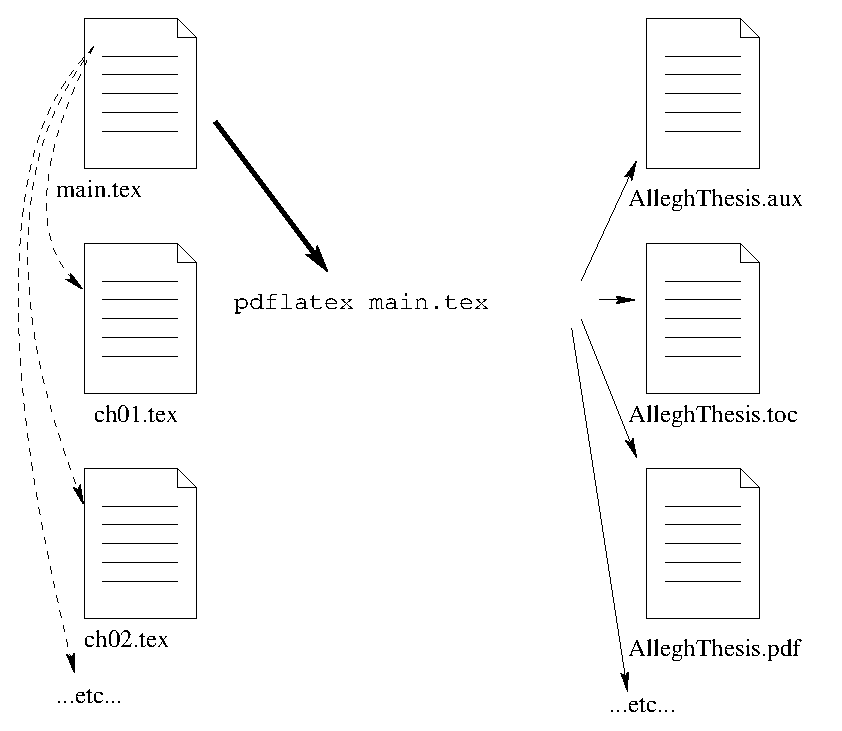
\includegraphics[width=3.5in]{latexprocess}
% % \caption{The first step in creating a thesis document}
% % \label{latexprocess}
% % \end{figure}
%
% \section{Current State of the Art}\label{sec:stateofart}
% There are multiple
% ways to create {\it italicized}, {\bf bold-face}, {\tt fixed-width}, and
% {\sf sans-serif} fonts, as well as combinations, e.g., \textit{\textbf{
% bold italic}} or \textit{\textsf{italic sans-serif}}. The \LaTeX\ source
% file for this chapter shows some of the ways to achieve these effects.
% It is customary to use fixed-width font for program constructs, e.g.,
% ``In the Java code accompanying the figure, {\tt n} stands for the
% number of generations to be simulated by the {\tt evolvePopulation()} method.''
% Variables in mathematical equations are normally rendered in
% italics, e.g., ``In the performance equation, {\it cpuTime} is
% the average time over fifty runs of the program.''
%
% %It is the privilege of the thesis author (in consultation with the
% %project supervisor and other readers) to decide on the best way to
% %organize the sections and chapters in the way that makes the most sense.
% %If the introduction begins with a motivating
% %anecdote, perhaps this is best followed by defining a few terms or mentioning
% %some major results that the reader should be aware of right from the
% %beginning. But
% It is important to get as quickly as possible to
% a concise statement of the {\it thesis}---the main question
% addressed by the project. This might merit a separate
% section of the chapter.
%
\section{Goals of the Project}\label{sec:goals}
% This section could also be entitled ``Thesis'' or something similar.
% A formal thesis statement should be a
% %\emph{falsifiable} % COMMENT OUT THINGS THAT YOU MAY LATER WISH TO PUT BACK
% statement about
% the goal achieved by the project.  For a purely scientific
% project, this is the hypothesis being tested; it should be a
% \emph{falsifiable} statement, i.e., one that can be disproven through
% an appropriate experiment.
% For an applied programming project, it is usually a statement about
% the feasibility and correctness of the approach used and the advantages it
% has over other approaches, using suitable metrics.  For a survey or study,
% it is usually a statement regarding the need
% or usefulness of such a study, its intended audience, and so on.
% % COMMENTED OUT NEXT FEW LINES TO SAVE SPACE; MAY PUT THEM BACK LATER
% %Following the concise statement of the thesis, some of the details can be
% %expanded.
% %It is appropriate to
% %refer to some of the results in the introduction (which may
% %mean going back and adding them to the introduction once the
% %research is completed).
% %A senior thesis, or any research paper, is not a mystery
% %novel---there is no need to keep the reader in suspense about what
% %has been accomplished.

Mnemosyne\footnote{Named for the Titaness who personified the concept of memory in Greek myth.} is a new programming language intended for systems programming. Mnemosyne is intended to reconcile the requirements of low-level systems implementation with the safety, expressive power, and elegance of modern functional programming languages.

\section{Thesis Outline}\label{sec:outline}

\Cref{ch:background} provides greater detail into the rationale behind Mnemosyne's creation and reviews preceding work in the area. \Cref{ch:design} discusses the considerations involved in the design of Mnemosyne's syntax and semantics, while \Cref{ch:implem} describes the implementation process for the prototype Mnemosyne compiler. In \Cref{ch:eval}, methods of evaluating the correctness of the Mnemosyne compiler prototype are discussed, and the results of these evalautions analyzed. Finally, \Cref{ch:conclusion} concludes this thesis with a summation of the outcomes of the research and a discussion of potential avenues for future work.
